\DiaryEntry{Elliptic Curve Cryptography}{2017-10-04}{Crypto}

Key exchange algorithms (like DHKE) require cyclic group as basis. One method is to use the groups $\mZ_p^\star$. Another option to obtain a cyclic group is to use elliptic curves. This entry gives a high-level overview of elliptic curves.

Consider a polynomial $p(x,y)$ and the corresponding equation $p(x,y) = 0$. This equation is solved by a set of points $(x,y)$. "Normally", these points are real numbers. As an example, consider $p(x,y) = x^2+y^2 - r^2$, then the equation becomes $x^2+y^2 = r^2$ and the points (taken from $\mR$) form a circle.

For cryptographic application, we need a finite set of points; therefore, we use $x,y \in \mZ_p$. The formal definition of an elliptic curve is defined as follows: 

\begin{definition}
	An elliptic curve over $\mZ_p$, $p > 3$, is the set of all pairs $(x,y) \in \mZ_p$ which fulfill
	\bee
	y^2 \equiv x^3 + ax + b \bmod p
	\eee
	together with an imaginary point $\Oc$ at infinity, where $a, b \in \mZ_p$ and the condition $4a^3 + 27b^2 \neq 0 \bmod p$.
\end{definition}

The condition ensures that the curve is non-singular; i.e. no self-intersections and or isolated points.

\subsubsection{Example}

An elliptic curve defined as above is difficult to visualize; however, we can plot an elliptic curve over the real numbers. A plot of $y^2 = x^3-3x + 3$is shown below.

\begin{figure}[H]
	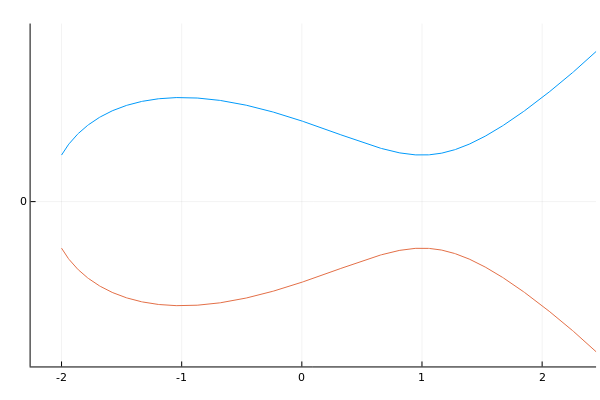
\includegraphics[scale=0.5]{images/elliptic_curves.png}
\end{figure}

The curve is symmetric around the x-axis (this is due to the fact that $y$ enters the equation only as $y^2$) and there is one intersection with the x-axis. An elliptic curve being a third-order equation, it has either one real solution (and two complex ones which are conjugate to each other) or three real solutions.

\subsection{Group Operations on Elliptic Curves}

In order to use elliptic curves for cryptographic purposes, we need to define a cyclic group structure on them. 

We denote the group operation with $+$; two points $P=(x_1, y_1), Q=(x_2, y_2)$ are combined into $R=(x_3, y_3)$. The coordinates $x_3, y_3$ are given by "some" equations (they are chosen in a way that the whole construct becomes a cyclic group); however, there is also a geometric interpretation which is given in the following.

\paragraph{Point Addition $P+Q$.} If $P\neq Q$, the point $R$ is obtained by drawing a line through $P$ and $Q$ in order to obtain a point at the intersection between the line and the elliptic curve. This point is mirrored along the x-axis which yields $R$. The Figure below shows the procedure. The only exception is when $P$ and $Q$ have the same $x$-coordinate. For this case, see further below.

\begin{figure}[H]
	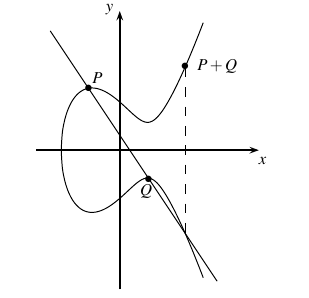
\includegraphics[scale=1.0]{images/elliptic_curves_groupop_1.png}
\end{figure}

\paragraph{Point Doubling $P+P$.} If $P = Q$, then a tangent at $P$ to the elliptic curve is drawn. This line intersects the elliptic curve at a point. By mirroring the interception point along the x-axis, the result $R$ is obtained.

The Figure below shows the procedure.

\begin{figure}[H]
	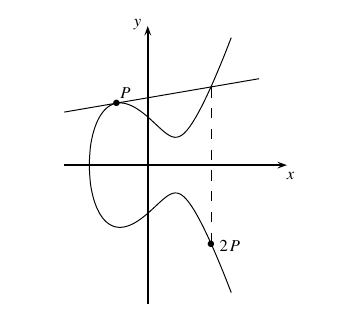
\includegraphics[scale=1.0]{images/elliptic_curves_groupop_2.png}
\end{figure}

We can write out above constructions using analytical expressions; in addition, we consider operations over the finite field $\mZ_p$ instead of real numbers. In this case, we obtain the following expressions

\begin{align*}
x_3 &= s^2 - x_1 - x_2 \bmod p \\
y_3 &= s(x_1-x_3) - y_1 \bmod p
\end{align*}

with the value $s$ as follows

\bee
s = \begin{cases}
	\frac{y_2 - y_1}{x_2 - x_1} \bmod p \qquad \text{if} P \neq Q \\
	\frac{3x_1^2+a}{2y_1} \bmod p \qquad \text{if} P = Q
\end{cases}
\eee

Be careful, the fractions above mean inverse $\bmod-p$; i.e. $(y_2 - y_1) (x_2 - x_1)^{-1} \bmod p$.

Up to now, we have no identity element $\Oc$. To this end we define an (abstract) point at infinity. This allows us to calculate the inverse of a point $P$:

\bee
P + (-P) = \Oc
\eee

and $-P$ is given by reflecting $P$ along the x-axis; i.e. $-P = (x_1, -y_1)$. We can use this result to add two points with the same $x$-coordinate: $(x_1,y_1) + (x_1,y_2)$: First note that $y_1 = -y_2$ because the elliptic curve is symmetric wrt to the $x$-axis. So we have $(x_1,y_1)+(x_1,-y_1) = \Oc$ following from the definition of the identity element.


\subsection{Cyclic (Sub)groups}

There is a theorem, which states that the points on an elliptic curve together with $\Oc$ have cyclic subgroups. Under certain conditions all points on an elliptic curve form a cyclic group.

\subsection{Example}

In the following, we will use the elliptic curve system $p = 17$, with $y^2 \equiv x^3 + 2x + 2$. I have implemented some stuff \href{https://github.com/ClemensFMN/JuliaStuff/blob/master/elliptic_curve_group.jl}{here} and used this in the following.

First consider the point $P = (5,1)$, doubling the point yields $2P = (6,3)$. By inserting $(6,3)$ into the elliptic curve equation, we can check that this is a valid point. The RHS equals $6^3 * 2\cdot 6 + 2 \equiv 9 \bmod 17$ and the LHS equals $3^2 = 9$. \qed

In order to investigate the group structure, we start with $P = (5,1)$ and calculate $2P, 3P, \ldots$. We obtain the following results



